\chapter{EVALUATION}

In this section, we will evaluate the performance of the key components of the system, the Information Extraction module and the Ontology Similarity module respectively, and then the whole system.

\section{Experiments of Information Extraction }

To evaluate the performance of information extraction module, we get some kinds sentences by the some sentence filters. We use the sentences that have degree information to explain the process of the experiment:

In the experiment, we selected 100 sentences from job descriptions, and the content of these sentences were requirements of candidates' degrees and majors. The values of degree and major are labeled manually. We use patterns to  match and extract the degree information from the sentences. The patterns are gotten from the observation of sentences. Figure~\ref{fig:degree_accuracy} shows that when the number of  patterns increases, the accuracy of information increases as well. When we used 6 patterns, the accuracy of degree became 94\%. We also compared our pattern matching method to conditional random fields (CRF) model~\cite{lafferty2001conditional}  based approach, which is a state of art machine learning model for sequence labeling. We used 200 sentences to train the CRF model, and features of CRF model are words in the sentences and part of speech tags of the words. The accuracies of information extraction of three fields with the two methods, pattern matching and CRF are shown in Table \ref{tab:ieaccura}

\begin{figure}[htbp]
  \centering
  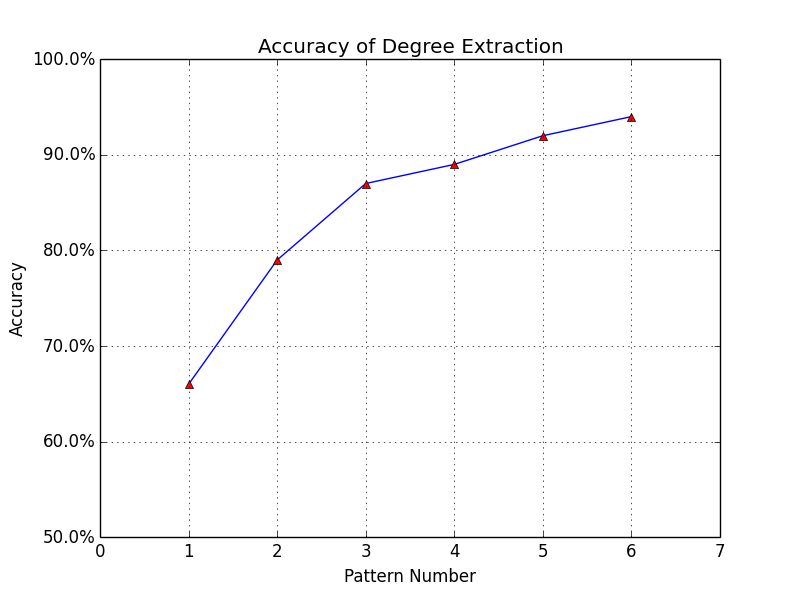
\includegraphics[scale=0.5]{images/degree_accuracy.png}
  \caption{Accuracy of Degree Extraction  }
  \label{fig:degree_accuracy}
\end{figure}


\begin{table}[ht]
\caption{Information Extraction} % title of Table
\centering % used for centering table
\begin{tabular}{   | c | c | c | c |   }
 \hline
          Field   & Pattern Num & Accuracy of Pattern Matching  & Accuracy of CRF   \\
 \hline
          Degree  & 6           & 0.94       &  0.85  \\
 \hline
          Major   & 10          & 0.85       &  0.72  \\
 \hline
          Skill   & 6           & 0.82       &  0.66  \\
 \hline
\end{tabular}
\label{tab:ieaccura} % is used to refer this table in the text
\end{table}

\section{Experiments of Ontology Similarity}

We selected some common skills from 500 job descriptions; table~\ref{tab:dismatrix3} shows similarity values between these skills. The values in the table are the similarities between skills, the higher the value, the greater the similarity, so the similarity between one skill and itself is 1. We selected one concept, ranked other concepts by their similarity values to this concept. The ranked concepts are also be given relevance scores by human judges, so we can use NDCG to evaluate the effectiveness of our approach.

\begin{table}

\caption{Similarities of Skill List 1}
\begin{tabular}{ c | c c c c c c   }
 \hline
  Term       &  Java  &  JDBC  & Spring & Hibernate & MySql  & Oracle   \\  \hline
  Java   &   1    & 0.0523 & 0.091  &   0.0458  & 0.0339 & 0.0608    \\  \hline
    JDBC   & 0.0523 &   1    & 0.0525 &   0.0799  & 0.006  & 0.0616   \\  \hline
   Spring  & 0.091  & 0.0525 &   1    &   0.2008  & 0.0194 & 0.0878   \\  \hline
 Hibernate & 0.0458 & 0.0799 & 0.2008 &     1     & 0.0073 & 0.115    \\  \hline
   MySql   & 0.0339 & 0.006  & 0.0194 &   0.0073  &   1    & 0.049    \\  \hline
   Oracle  & 0.0608 & 0.0616 & 0.0878 &   0.115   & 0.049  &   1      \\  \hline
 \hline
\end{tabular}
\label{tab:dismatrix3}
\end{table}

We use $ Normalized~Discounted~Cumulative~Gain ( NDCG )$ to evaluate the statistical-based similarity. NDCG is an important measure to evaluate the ranked retrieval results. For a set of queries $Q$, let $R(j,d)$ be the relevance score assessors gave to document $d$ for query $j$.
       $$ NDCG(Q,k) = \frac {1}{|Q|} \sum_{j=1}^{|Q|}{Z_{kj}} \sum_{m=1}^{k} \frac{2^{R(j,m)} - 1}{ \log_2(1+m)} $$

Where $Z_{kj}$ is a normalization factor calculated to make it so that a perfect ranking's NDCG at $k$ for query $j$ is 1. For queries for which $k' < k$ documents are retrieved, the last summation is done up to $k'$.

Table ~\ref{tab:simcompare1} shows how we evaluate the similarity between the concept ``Javascript'' and some other concepts. The first column is some skill names, the second column is their similarity values to Javascript, the third column is their positions ranked by the similarity values, and the fourth column is their relevance values given by the judges. The NDCG value for concept Javascript is 0.94, and in table ~\ref{tab:simcompare2},  NDCG value for concept HTML is 0.97.

\begin{table}
\centering
\caption{ Javascript Similarity Evaluation : NDCG = 0.94 }
\begin{tabular}{ | c | c | c  | c |  }
 \hline
    Term     &  Similarity Value  &  Position   & Relevance     \\  \hline
    jQuery   &  0.1981            &      4      &   8        \\
     HTML    &  0.2087            &      3      &   4         \\
     CSS     &  0.2439            &      2      &   3   \\
     Java    &  0.0665            &      5      &   1   \\
    Python   &  0.0189            &      8      &   1   \\
     Ruby    &  0.023             &      7      &   1    \\
     JSP     &  0.0253            &      6      &   2    \\
 \hline
\end{tabular}
\label{tab:simcompare1}
\end{table}


\begin{table}
\centering
\caption{ HTML Similarity Evaluation : NDCG = 0.97 }
\begin{tabular}{ | c | c | c  | c |  }
 \hline
    Term      &  Similarity Value  &  Position   & Relevance     \\  \hline
  Javascript   &  0.2087           &      2      &   3        \\
     jQuery    &  0.0979           &      3      &   3         \\
     CSS     &  0.3569             &      1      &   5   \\
     Java    &  0.0473             &      4      &   1   \\
    Python   &  0.0175             &      6      &   1   \\
     Ruby    &  0.023              &      5      &   1    \\
     JSP     &  0.0103             &      7      &   3    \\
 \hline
\end{tabular}
\label{tab:simcompare2}
\end{table}


\section{Evaluation of the System}

In traditional information retrieval systems, precision and NDCG are widely used measures ~\cite{manning2008introduction}. Precision ($P$) is the fraction of retrieved documents that are relevant .
       $$  Precision =  \frac{ \#(releveant~items~ retrieved)}{ \#(retrieved~items)}$$

We first used Precision@K to compare the performance our approach to some classical information retrieval models, that are Okapi BM25~\cite{robertson2009probabilistic}, Kullback-Leibler divergence, and the TF-IDF. Precision@K is the proportion of relevant documents in the first K positions and is given below:
$$ P@k = \frac{1}{k} \sum^m_{i=1} l_i 1 \left(  r(i) \leq k  \right )  $$
Where 1 is the indicator function: $1(A) = 1$ if A is true, 0 otherwise.

To evaluate job finding, we compare the results of the system with three classical information retrieval models: Kullback-Leibler divergence~\cite{zhai2008statistical},  TF-IDF~\cite{manning2008introduction} and Okapi BM25 ~\cite{robertson1995okapi}. We give the definition these measures as below.

Kullback-Leibler divergence is a non-symmetric measure of the difference between two probability distributions $P$ and $Q$. The score of a document $D$ with respect to query $Q$ is given by:
\begin{equation}
    \begin{array}{rcl}
        s(D,Q) & = & -D( \theta_Q \parallel  \theta_D )\\
               & = &- \sum_{ \omega \in V } p (\omega \mid \theta_Q) \log \frac{ p (\omega \mid \theta_Q )}{p(\omega \mid \theta_D)} \\
               & = & \sum_{ \omega \in V } p (\omega \mid \theta_Q) \log p (\omega \mid \theta_D ) -  \sum_{ \omega \in V } p (\omega \mid \theta_Q) \log p (\omega \mid \theta_Q )  \\

    \end{array}
\end{equation}

In the equation $\theta_Q$ is language model for a query, and  $\theta_D$ is language model for a document.

TF-IDF is a Vector Space Model, which calculate Cosine Similarity between the vectors of the query $q$ and the document $d$. In the equation, $tf$ is term frequency, and $idf$ is inverse document frequency. The tf-idf weighting scheme assigns to term $t$ a weight in document $d$ given by:
$$ tf\text{-}idf_{t,d} = tf_{t,d} \times idf_{t} $$
The similarity between the  the query $q$ and the document $d$ given by:
$$ score(q,d) =  \sum_{t \in q }  tf\text{-}idf_{t,d} $$

Okapi BM25: Given a query $Q$, containing keywords $q_1, ..., q_n$, the BM25 score of a document $D$ is:

$ score(D,Q) = \sum_{ i=1 }^{n} IDF(q_i) \cdot   \frac {f(q_i,D) \cdot (k_1 + 1)}{f(q_i,D) + k_1 \cdot ( 1-b + b\cdot \frac { \left | D \right |}{avgdl})}  $

In the evaluation phase, we created a data set of 100 job descriptions, which includes several kinds of jobs, like web developers, back-end developers, mobile developers and so on. We used 5 candidate r\'esum\'es and retrieved the top 20 jobs.  The relevance value of job descriptions to each r\'esum\'e will be set manually. We create a query q from the r\'esum\'e, and treat the text of the job descriptions as documents d and apply standard ad-hoc retrieval techniques to rank the jobs. We would like to return jobs that better match the candidates' r\'esum\'es at the top. The result of Precision@k is in table~\ref{tab:job_precision}.


\begin{table}[ht]
\caption{Precision of Job Ranking } % title of Table
\centering % used for centering table
\begin{tabular}{    | c | c | c | c | c |  }
 \hline
       k     & Okapi BM25 & KL    & TF-IDF   & Ontology Similarity  \\
 \hline
       5     & 0.13       & 0.40  & 0.54     & 0.74   \\
 \hline
       10    & 0.16       & 0.36  & 0.50     & 0.66   \\
 \hline
       20    & 0.16       & 0.35  & 0.49     & 0.61   \\
 \hline

\end{tabular}
\label{tab:job_precision} % is used to refer this table in the text
\end{table}

The other measure we used is NDCG, which is explained in last section. Table ~\ref{tab:job_ndcg} shows the NDCG value get from different information retrieval models. The result shows that Ontology Similarity  performs the best.

\begin{table}[ht]
\caption{NDCG of Job Ranking } % title of Table
\centering % used for centering table
\begin{tabular}{    | c | c | c | c | c |  }
 \hline
       k    & Okapi BM25 & KL    & TF-IDF & Ontology Similarity  \\
 \hline
       5    & 0.15       & 0.34  & 0.45     & 0.78   \\
 \hline
       10   & 0.18       & 0.44  & 0.47     & 0.72   \\
 \hline
       20   & 0.19       & 0.35  & 0.45     & 0.66   \\
 \hline

\end{tabular}
\label{tab:job_ndcg} % is used to refer this table in the text
\end{table}

